\documentclass{beamer}
\usetheme{Boadilla}

\usepackage{amsmath}
\usepackage{amsfonts}
\usepackage{hyperref}

\usepackage{amsmath}
\DeclareMathOperator*{\argmax}{arg\,max}
\DeclareMathOperator*{\argmin}{arg\,min}

\title{BANANAS: Bayesian Optimization with Neural Architectures for Neural Architecture Search
}
\author{Galina Boeva}
\institute{MIPT, 2023}


\begin{document}

\begin{frame}
    \titlepage
\end{frame}


\begin{frame}
    \tableofcontents
\end{frame}


\section{Motivation}
\begin{frame}{Motivation}
    \begin{block}{Main idea}
    NAS algorithms are now common. But the analysis in the papers often focuses on a full-fledged NAS, so it is difficult to say which individual components of the framework provide the best performance. Therefore, it is interesting to consider the individual components of the framework.
    \end{block} 

    \begin{figure}
        \centering
        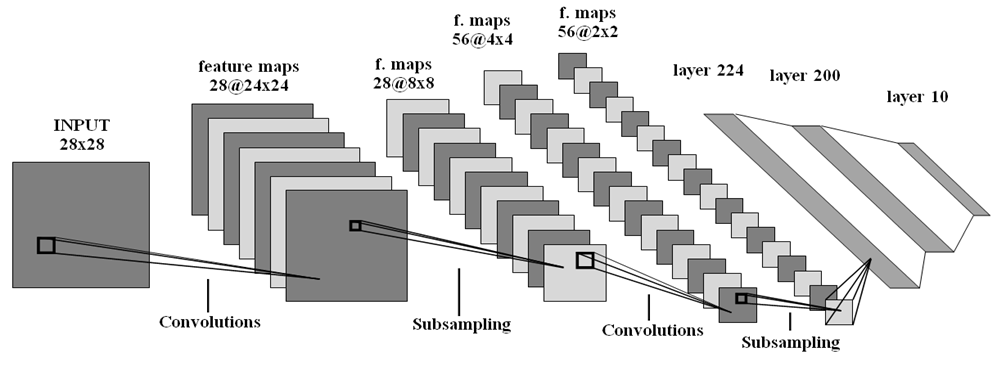
\includegraphics[scale=0.45]{images/svertka.png}
        %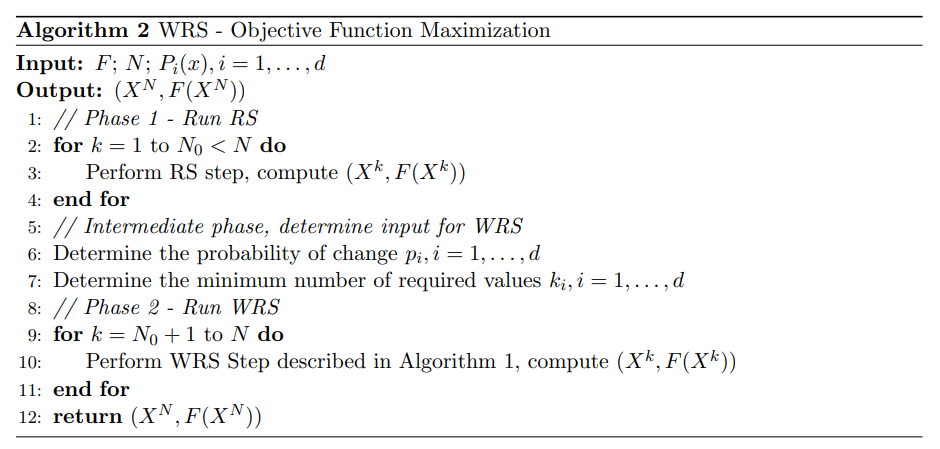
\includegraphics[scale=0.5]{images/wrs2.png}
        \label{fig:enter-label}
    \end{figure}
    
\end{frame}


\section{Analysis of the Framework}
\begin{frame}{BO + Neural Predictor Framework}
%\centering
Consists of 4 components:
\begin{itemize}
    \item Architecture encodings
    \item Neural predictors
    \item Uncertainty calibration
    \item Acquisition functions and optimization
\end{itemize}

\end{frame}

\begin{frame}{Analysis of the Framework: path
encoding}
\centering
\begin{figure}
        \centering
        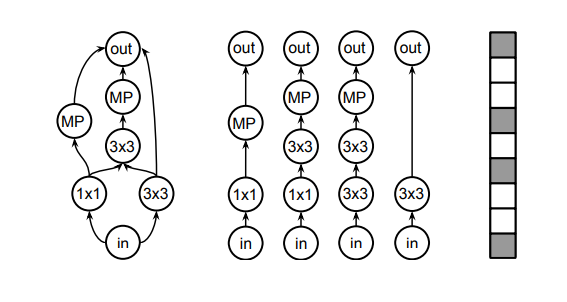
\includegraphics[scale=0.55]{images/bananas7.png}
        %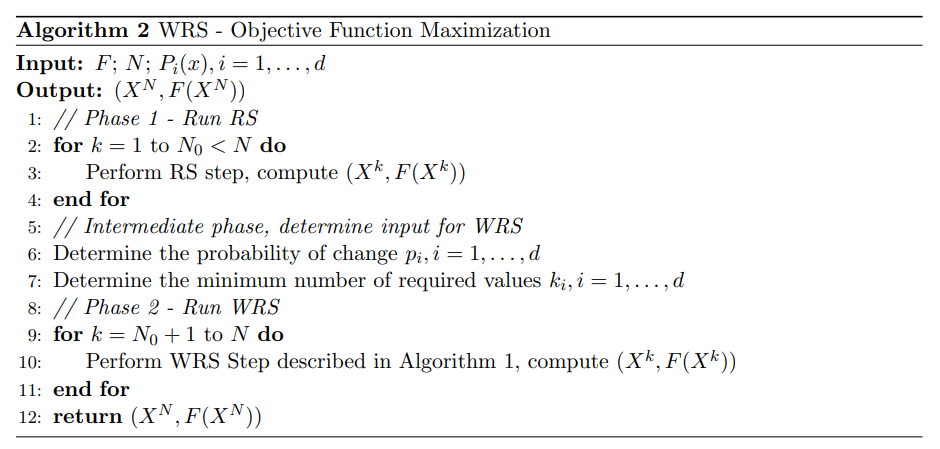
\includegraphics[scale=0.5]{images/wrs2.png}
        \label{fig:enter-label}
    \end{figure}
    \begin{figure}
        \centering
        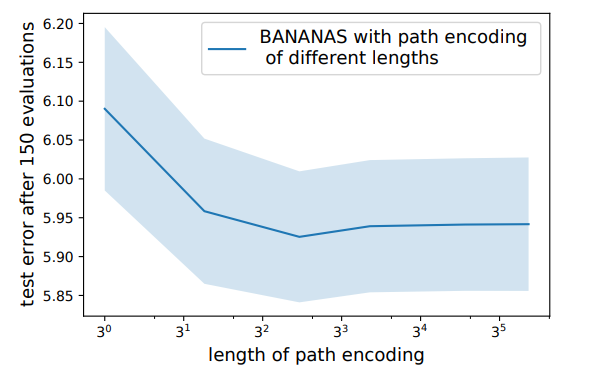
\includegraphics[scale=0.55]{images/bananas6.png}
        %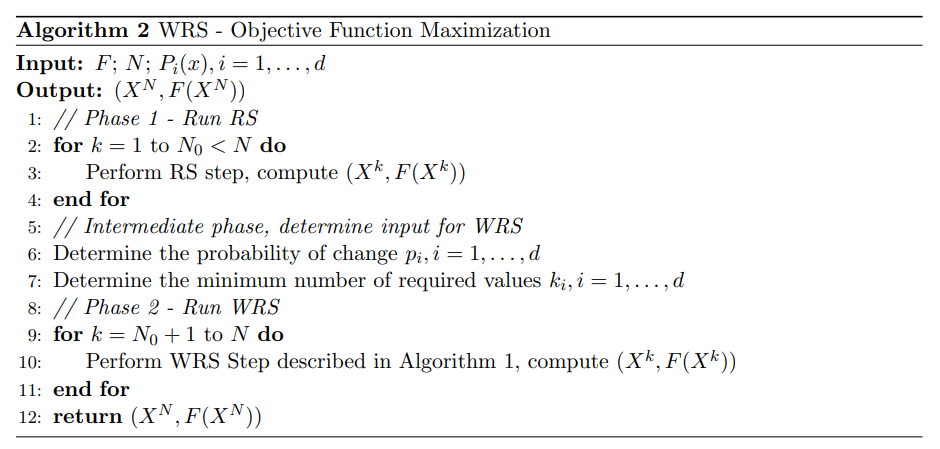
\includegraphics[scale=0.5]{images/wrs2.png}
        \label{fig:enter-label}
    \end{figure} 
\end{frame}


 
\end{frame}

\begin{frame}{BANANAS}
\centering 


\begin{figure}
        \centering
        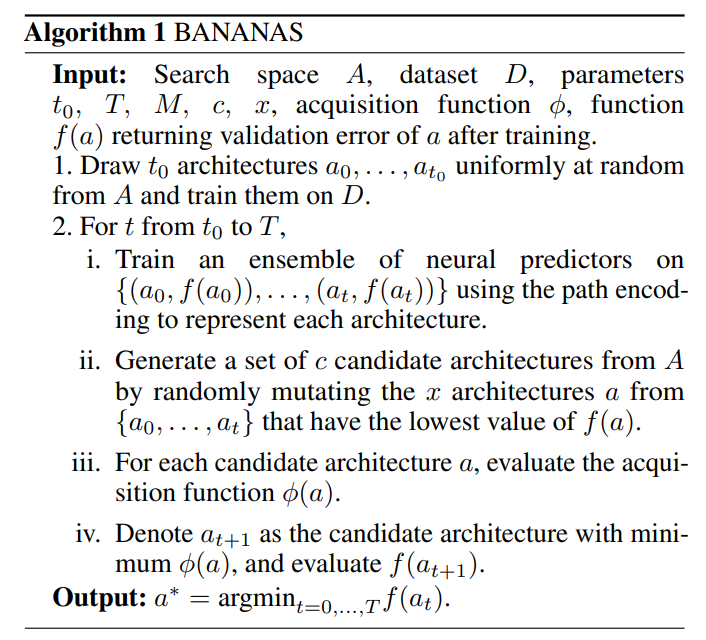
\includegraphics[scale=0.7]{images/bananas1.png}
    \end{figure}
 
\end{frame}


\section{Experiments of BANANAS}
\begin{frame}{Experiments of BANANAS}
    \begin{figure}
        \centering
        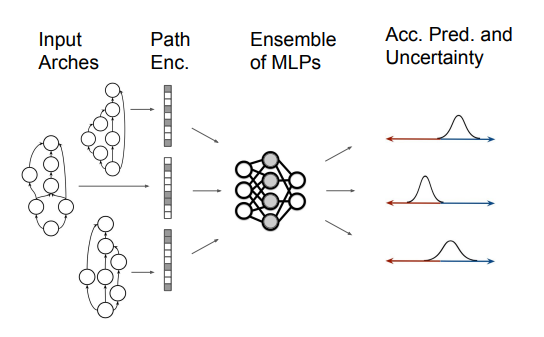
\includegraphics[scale=0.6]{images/bananas2.png}
    \end{figure}
    \begin{figure}
        \centering
        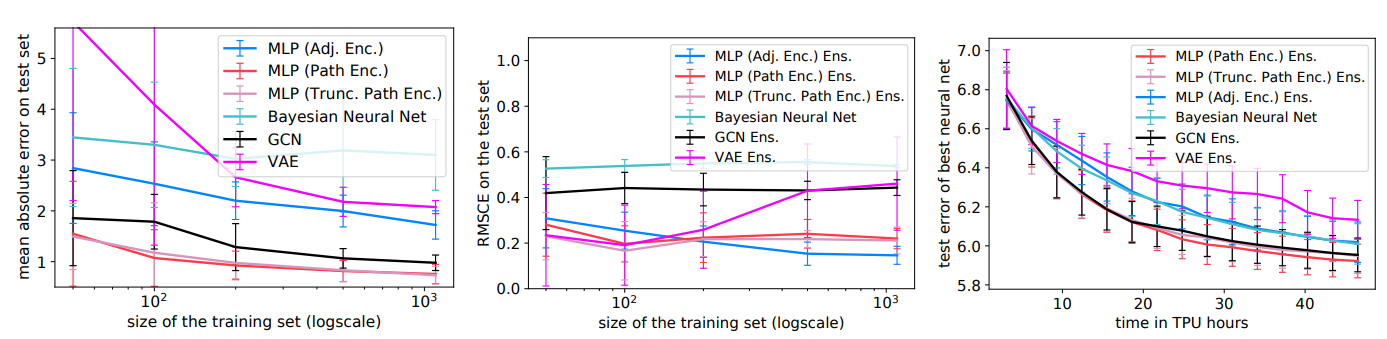
\includegraphics[scale=0.5]{images/bananas5.png}
        \caption{Performance of neural predictors.}
        \label{fig:enter-label}
    \end{figure}
\end{frame}
\begin{frame}{Experiments of BANANAS}
    \begin{figure}
        \centering
        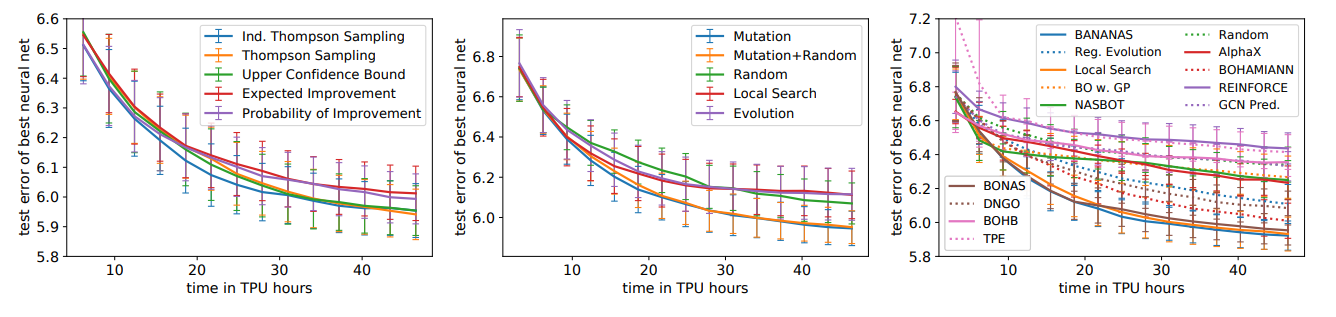
\includegraphics[scale=0.5]{images/bananas3.png}
        \caption{Performance of different acquisition functions, different acquisition function optimization strategies, other NAS algorithms.}
        \label{fig:enter-label}
    \end{figure}
    \begin{figure}
        \centering
        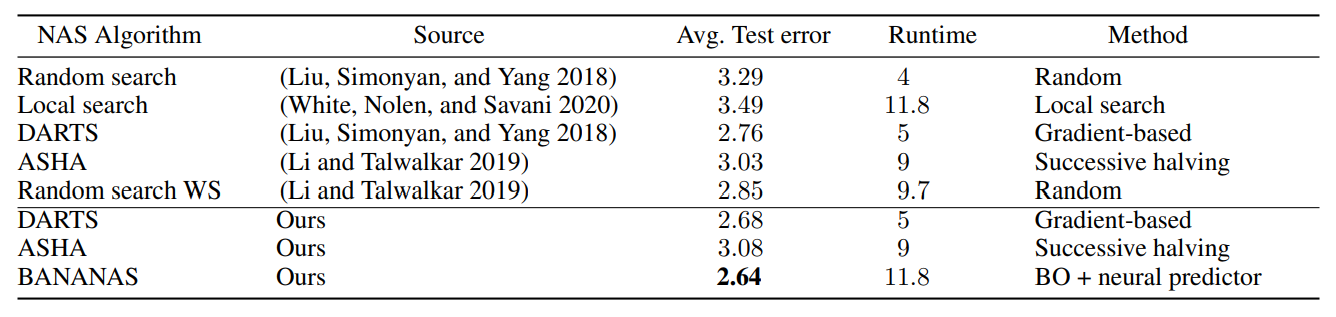
\includegraphics[scale=0.5]{images/bananas4.png}
        \caption{ Comparison of NAS algorithms on the DARTS search space.}
        \label{fig:enter-label}
    \end{figure}
\end{frame}
 


\begin{frame}{Literature}
    \begin{enumerate}
        \item \textbf{Main article} \href{https://arxiv.org/pdf/1910.11858.pdf}
        {BANANAS: Bayesian Optimization with Neural Architectures for Neural Architecture Search}.
    \end{enumerate}
\end{frame}



\end{document}